\section{Morphological quantification of filamentous microbes}

Many attempts have been made to express the product yield from an organism in a given process in terms of the morphological form adopted \cite{papagiannireview}. Of fundamental importance to the elucidation of such relationships is the ability to accurately and unambiguously quantify structural variation in microbial conformations. Early investigations involved the manual measurement of morphological features either directly using a microscope (and a graticule, for example) or indirectly by photography. Trinci studied the growth kinetics of various filamentous moulds by imaging cellophane-immobilised cultures (to restrict growth to two dimensions) in inverted Petri dishes with a 35~mm camera and then taking manual measurements from enlarged prints \cite{trinci1974}. Although extensive data (total hyphal length and number of tips versus time, specific growth rate, specific branching rate and mean tip extension rate) was presented on the development of \emph{G. candidum}, \emph{A. nidulans}, \emph{M. hiemulis}, \emph{P. chrysogenum} and \emph{N. crassa}, such a procedure would be extremely laborious and time-consuming, even with modern digital cameras, meaning only a small number of mycelia could be studied (3 -- 5 per organism in the case of Trinci).

\subsection{Development of image processing systems for mycelial analysis}

The application of image processing, defined as \lq \emph{the conception, design, development and enhancement of digital imaging programmes}' \cite{burger2008}, to the study of filamentous microbes was, until recently, limited by the available computer hardware - many \lq personal computers' of the late 1980's were not equipped with the necessary capability to load into memory a single image from a modern digital camera. Image processing has clear advantages in terms of speed and lower labour intensity and imaging systems also have the potential to be automated, reducing the workload still further and permitting online analysis of samples. Digital images may also be transferred electronically to a location remote from the laboratory for analysis if required.

A typical imaging system utilised for the quantification of fungal morphology might consist of a standard bright-field microscope onto which a digital camera is mounted. Studies employing image analysis techniques often mounted video cameras on microscopes and then captured images on a PC by way of a frame-grabber \cite{bartnicki-garcia2000,li2000}. However, the proliferation of universal serial bus-enabled devices largely negates the need for such a set-up in the modern laboratory. Once the image has been transferred to the PC, some form of image processing application is required to extract the relevant data. There are commercially available image processing packages that may be used for this task, but many are expensive and are not application-specific. Alternatively, open-source applications such as ImageJ \cite{imagej} may be extended by way of plug-ins, permitting the user to adapt the pre-existing functionality of the application to their needs, or incorporate wholly original algorithms as is necessary. Considerations of computer specifications, such as processor speed and memory capacity, are also now largely unnecessary, as a typical desktop or laptop PC will almost certainly be equipped with the necessary functionality to run most image processing tasks.

The first attempts to represent filamentous microbes digitally were described by Metz and colleagues, who projected magnified images of mycelia onto a digitising table (graphics tablet) \cite{metz1981}. Touching a point on the digitiser with stylus caused the $(x,y)$ coordinates of that point to be output to an attached computer (IBM 1130), which estimated the length of a hypha by calculating the distance between this series of points (Fig.~\ref{fig:Fig2Metz1981}). The particle dimensions were subsequently output (punched on paper tape) by the computer and fed into an IBM mainframe (370-158) for statistical analysis. Extensive data was presented on morphological parameters such as main hyphal length ($\Lm$), total hyphal length ($\Lh$) and the hyphal growth unit ($\hgu$). However, the method was very time-consuming and labour-intensive, permitting the examination of a relatively small population (10 -- 20 mycelial elements per sample), resulting in large errors in the estimation of parameter means in an assessment of the development of \emph{P. chrysogenum}. Furthermore, mycelial clumps were not considered due to their complexity and measures of hyphal diameter were unreliable, due to the poor resolution of the digitiser. Nevertheless, this represented an important step toward the digital quantification of filamentous microbes.

\begin{figure}[t]
	\centering
	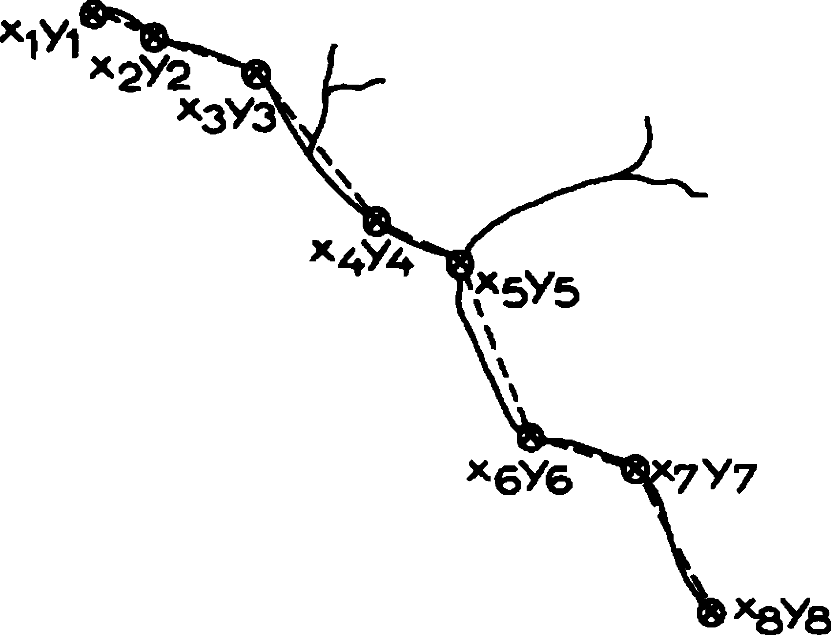
\includegraphics[width=8cm]{../C1/Fig2Metz1981}
	\caption{Calculation of hyphal length by means of a digitising table according to Metz and colleagues \cite{metz1981}. Reproduced with permission from John Wiley and Sons.}
	\label{fig:Fig2Metz1981}
\end{figure}

%A manual image analysis method was later described by Wiebe and Trinci to quantify the morphology of \emph{Fusarium graminearum} \cite{wiebe1991}. Images were transferred to a computer from a digital camera and measures of main hyphal length, total hyphal length and hyphal diameter were made by tracing the images.

Martin and Bushell proposed an alternative method for the quantification of hyphal fragments of \emph{S. erythraea}, which involved circumscribing a circle around each object in an image \cite{martin1996}. The diameter of the circle was then interpreted as the \lq maximum diameter' of a hyphal fragment. Stained slides were imaged with a phase-contrast microscope and the resulting photographs were examined using a stencil containing circles of various diameters; the maximum mycelial diameter was determined as the diameter of the smallest circle that completely enclosed the object. It may be possible to automate such a procedure, but fitting circles around irregular objects such as mycelia would be computationally expensive and the net benefit of the maximal diameter parameter over conventional measures such as projected area is questionable.

The first significant advance on the digitising table method was proposed by Adams and Thomas, who described a semi-automatic image processing system to derive similar measurements of hyphal filaments \cite{adams1988}. The performance of their image analysis system was compared to that of a digitising method, similar to that described by Metz and colleagues \cite{metz1981}. Manual editing of the binary images produced by the imaging system was necessary (elimination of artifacts, separation of branches from main hypha) and although the total time required to quantify a single hyphal element was substantial by modern standards (approximately 1~minute), the digitising method was estimated to be up to five times slower. Furthermore, image processing was shown to be more accurate for the determination of hyphal lengths, as \lq arcs' in the hyphae were more accurately represented and the subjectivity surrounding the location of branch-points was removed. Image processing was also far more convenient, as it obviated the requirement for photographic film development.

Packer and Thomas later described a fully-automated system that produced similar metrics, but also considered \lq clumped' biomass for the first time \cite{packer1990}. The program (implemented on a Magiscan 2A image analyser) required the manual setting of certain application-specific parameters: a grey-level threshold for image segmentation, a circularity threshold, the specification of a \lq measuring frame' to exclude truncated structures at the image boundary and a maximum length threshold for the identification of artifactual branches (caused by debris). Once these parameters were established, the system proceeded automatically to segment the input image (to produce a binary image), eliminate artifact using a circularity test and skeletonise the remaining objects. The dimensions of each hyphal element were subsequently evaluated ($\Lm$, $\Lh$, $N$ and $\hgu$) and the percentage of clumped material was also calculated (clumps were identified as relatively circular objects containing \lq holes'). The results produced by the automated system, on the development of \emph{Streptomyces clavuligerus} in submerged culture, were in close agreement with those produced using a manual image processing method, which involved manual editing of binarised images (filling \lq false' holes, eliminating hyphal crossovers, removing debris) and manual selection of mycelia. However, the automated method was only marginally faster than the manual method. This was attributed to the time-consuming nature of the skeletonisation algorithm, but employing modern hardware should alleviate this problem. Furthermore, it was demonstrated that the percentage of biomass present in the form of clumps in a given sample was dependent on sample dilution, which tended to disperse entangled mycelia. Given this sensitivity, it was concluded that proportion of material present in the form of clumps may not be a reliable morphological indicator, unless excessive dilution was employed and long processing times were acceptable. However, subsequent studies have utilised analysis systems that extracted similar metrics to those described above \cite{elsabbagh2006}.

%It is possible that the branching behaviour within clumps (and pellets) may be inferred from an analysis of free mycelial elements \cite{cox1998}, but an analysis of the clumped morphology is still required given the implications for rheological performance of the fermentation broth and subsequent impacts on productivity \cite{znidarsic2001}. There also exists the possibility that a process may consist almost exclusively of the pelleted or clumped morphology, in which case the analysis of free elements to characterise the morphology cannot be relied upon.

Tucker and colleagues expanded upon the work of Packer and Thomas by including measures of clump \lq roughness' (circularity) and \lq fullness' (ratio of projected area to convex area) \cite{tucker1992}. The set-up (on a Leica Quantimet 570) used was similar to that described by Packer and Thomas. Following image segmentation and the production of a binary image, artifacts were removed using a combination of morphological (\lq opening') and size/circularity thresholds. Clumps were identified by \lq ultimate skeletonisation'; successive removal of pixels until either a single point or a \lq loop' (resulting from a background region enclosed within an object, characteristic of clumps) remained. In addition to projected area and perimeter (both determined by pixel counts), clumps were characterised in terms of circularity and compactness, which was measured in two ways: the ratio of pixel area to total area enclosed by the perimeter and the ratio of area to convex area ($A_c$; area enclosed by convex perimeter). Following the removal of small, \lq artificial' branches, free hyphal elements were subjected to a \lq shrink-back' algorithm, involving the iterative \lq pruning' of mycelia to identify branch-points, to classify branches as zero-order, first-order, and so on. This permitted a more detailed examination of mycelial structures beyond the conventional hyphal growth unit. However, this additional processing resulted in a substantial increase in execution time from approximately 41~seconds per field of view (Packer and Thomas) to 67~seconds. However, subsequent studies have employed the same methodology to extract similar features to those described above \cite{mcintyre1998,amanullah2000,li2000}.

The method of Tucker and colleagues was further improved upon by Paul and Thomas \cite{paul1998}. The production of a skeletonised image was performed as described by Tucker and colleagues, with remaining artifacts removed based on an evaluation of the \lq fullness' ratio ([projected area prior to skeletonisation]/[convex area]), which was typically lower for mycelia. Mycelial trees were then quantified according to $\Lh$, $N$, $A$, branch order and length and inter-nodal distances; similar measures were applied to \lq simple' clumps or loose entanglements (clumps containing only 1 -- 3 \lq holes', resulting from hyphal crossovers). Clumps were analysed on the basis of maximum dimension, roughness, fullness ratio and area. The system was used to monitor the development of \emph{P. chrysogenum} in submerged fermentation and it was found that a significant reduction in clump size occurred from 24~hours post-inoculation, in tandem with a reduction in the total length of and number of tips per free mycelial element. It was postulated that this may have been partly a result of hyphae being sheared off the periphery of clumps.

A more complete description of clumped morphology was proposed by Papagianni and colleagues \cite{papagianni1994}. The perimeter of mycelial clumps ($P1$) was measured by joining the tips of the filaments that arose from the core of the clump. The perimeter of the clump core ($P2$) was estimated by drawing lines around the core and measuring their length. The total length of filaments and their branches that arose from the core ($l$) were also measured, although how this was achieved was not specified. Furthermore, the high degree of entanglement at the core periphery made it impossible to distinguish between main filaments and their branches and it was therefore suggested that $l$ indicated the degree of branching. However, precisely what dimension $l$ corresponded to was not made clear. The hyphal diameter ($d$) was also determined, by joining two opposite points on the hyphal wall and estimating the distance. The image analysis method was described as automatic, although based on the description, it would appear that significant manual intervention was required.

One of the limitations associated with the systems described above is the inability to analyse the ultra-structure of mycelial trees while simultaneously extracting information on hyphal width from the same image. This difficulty stems from the considerable difference in scale between the width of a hypha and the width of a mycelium (2 -- 3 orders of magnitude). A possible solution to this problem may be the use of a motorised stage to construct a matrix of high-resolution images, such as that which was employed by M\"{u}ller and colleagues to extract information on septum and nuclei positions in \emph{A. niger} and \emph{A. oryzae}, while also quantifying large hyphal arrangements using the same set of images \cite{muller2000}. Samples were stained with calcofluor white and 4',6-diamidino-2-phenylindole\footnote{DAPI: a nucleic acid stain, which binds strongly to DNA, used in multicolour fluorescent techniques.} then imaged with a $\times 100$ objective. By forming a $9 \times 9$ array with the resultant images, a sufficient resolution was obtained to simultaneously visualise sub-cellular details and ultra-structural variation, although significant user intervention was required, with distances between the apical tip, nuclei and septae all measured manually.

\subsubsection{Online monitoring of mycelial development}

One of the principal advantages of image processing systems is their potential use in conducting online assessment of hyphal extension, whereby images may be routinely captured and analysed automatically in tandem with development. Spohr and colleagues described such an online system \cite{spohr1998} based on a small \lq flow-through cell', consisting of a microscope slide above a Perspex base, separated by a Parafilm{\texttrademark} spacer, mounted on a microscope stage (Fig.~\ref{fig:Fig1Spohr1998}). Liquid media was pumped through an inlet valve on one side of the cell and removed through another. By fixing fungal spores to the inside of the slide (using Poly-{\scshape d}-lysine) and circulating nutrient media through the cell, the growth of the organism could be monitored using phase-contrast optics.

The data produced by Spohr and colleagues on the development of \emph{A. oryzae} mycelia was similar to that produced earlier by Trinci \cite{trinci1974} (albeit with a greater number of data-points), permitting the calculation of the specific growth rate and branching rates. In general agreement with the work of Trinci, it was found that the extension rates of different branches within a single mycelium varied, with the extension rate postulated to be proportional to the position of the branch relative to the primary tip. Evidence was also presented for the secretion of growth-stimulating compounds by \emph{A. oryzae}; high flow rates resulted in poor growth, which was not evident when \lq recycled' media was used. In addition, Spohr and colleagues presented data on the swelling of spores; circularity remained approximately constant during the swelling process, while measures of projected area over time suggested that spore volume increased exponentially prior to germination.

\begin{figure}[tb]
	\centering
	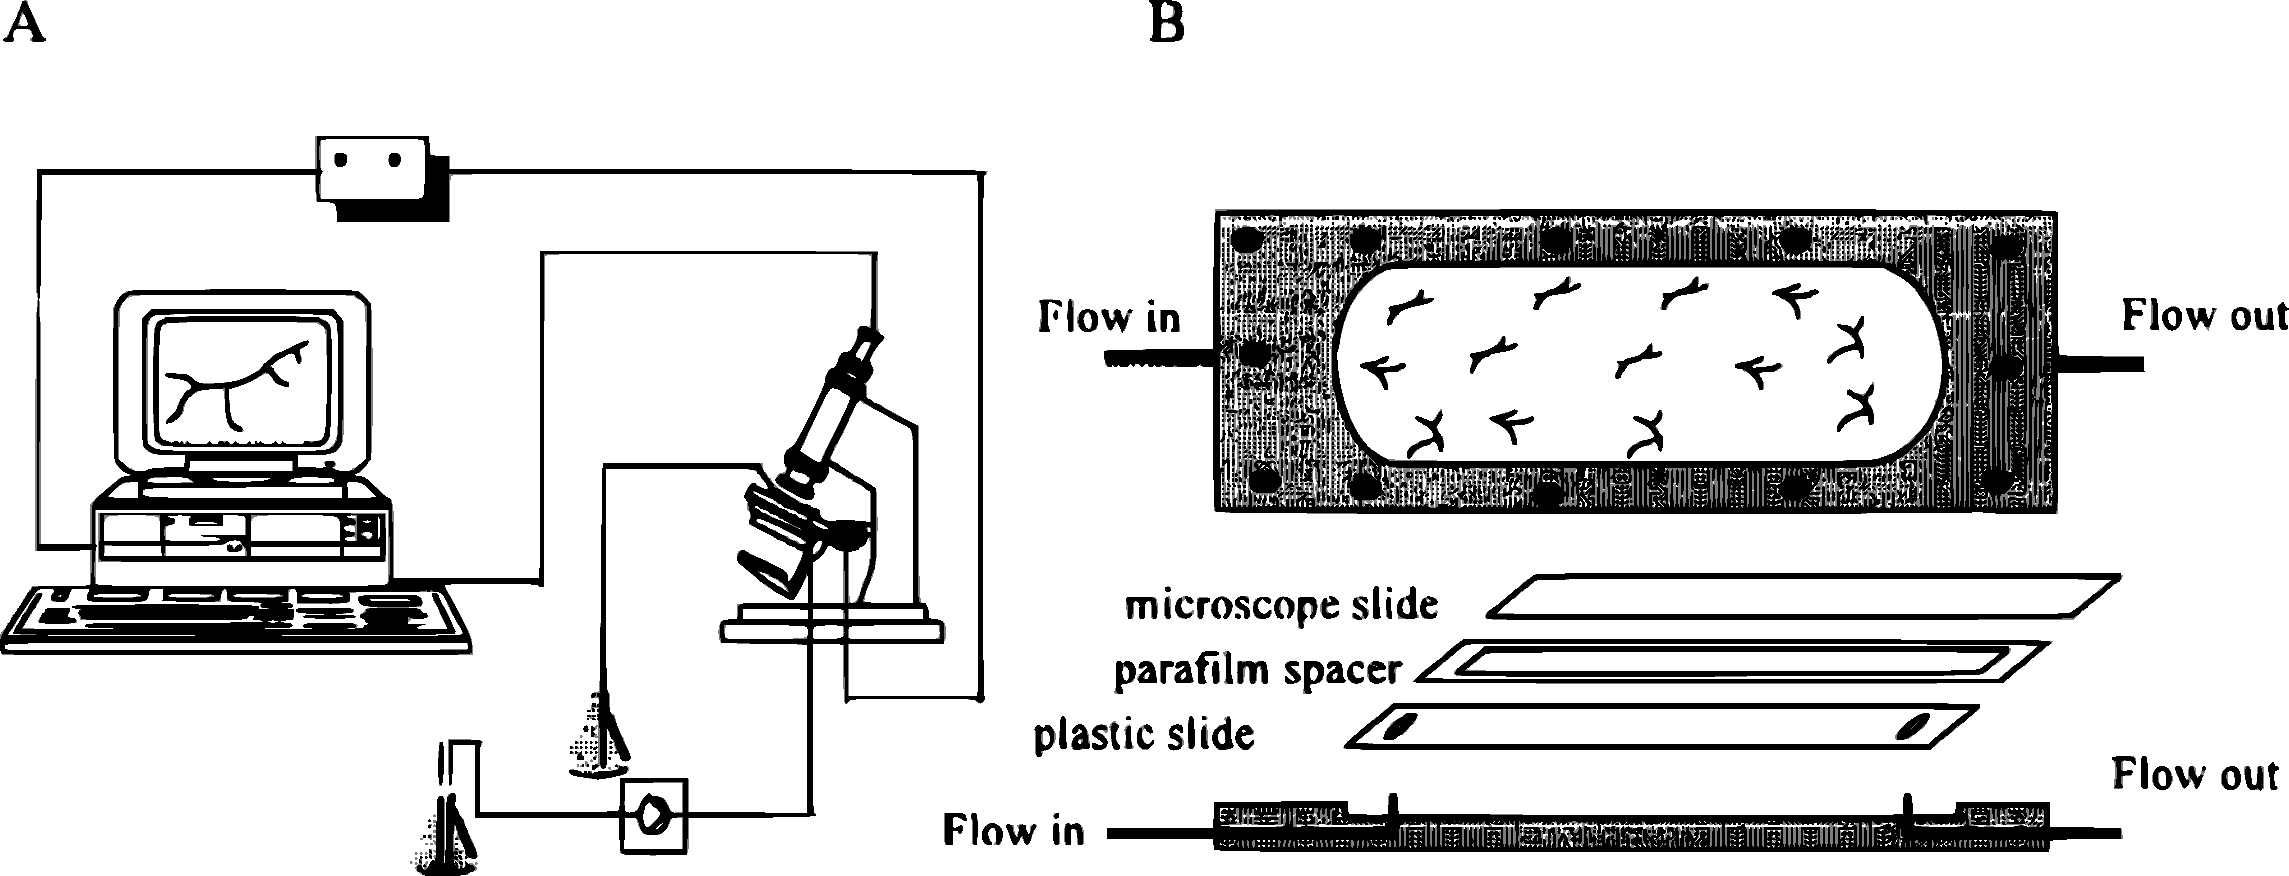
\includegraphics[width=(\textwidth - 1cm)]{../C1/Fig1Spohr1998}
	\caption{Schematic of the online imaging system employed by Spohr and colleagues \cite{spohr1998}. {\bf A.} The system consisted of an image analyser, a CCD-camera, a phase-contrast microscope and a flow-through cell mounted on the microscope, all of which were enclosed in a thermostated cupboard to ensure a constant temperature. The temperature sensor was located in the proximity of the chamber. {\bf B.} Construction of the flow-through cell. Reproduced with permission from John Wiley and Sons.}
	\label{fig:Fig1Spohr1998}
\end{figure}

The advantage of such a system is the ability to monitor the growth of individual elements, and even individual hyphae, from a single spore, up to a mycelium several millimetres in length. However, the methodology employed by Spohr and colleagues was perhaps slightly inefficient; analysis of images was conducted post-cultivation rather than simultaneously, requiring the use of a storage device for the large number of images captured. Quantification of morphological parameters post-cultivation was necessary as user intervention was required to identify the formation of a new branch in the image sequence for each mycelium, resulting in increased processing time. Similar systems have since been used to assess the development of \emph{Mucor circinelloides} \cite{lubbehusen2003,lubbehusen2004} and various \emph{Mortierella} species \cite{eypark2002,eypark2006}.

%However, some studies have attempted to identify other morphological parameters of interest. Yang and colleagues devised a system for the determination of branching angles and found that, within a population, branching angles were normally distributed. A model was proposed which predicted the development of the organism up to the pelleted form \cite{yang1992}.

\subsubsection{Sub-cellular analysis}

A limited number of studies have focussed on the analysis of sub-cellular hyphal features. Paul and Thomas developed one such system, designed to quantify vacuolation and \lq active' growing regions in neutral red-stained \emph{P. chrysogenum} mycelia \cite{paul1998}. Their elegant routines comprised a series of grey-scale and binary morphological operations to extract vacuoles and active hyphae from an image, although some manual editing was required. The objects of interest (hyphae, vacuoles, active tips) all exhibited different grey levels and each could be segmented from the input image using different grey-level thresholds. Artifacts in the resulting binary images could generally be identified based on size and circularity. Their results showed that the percentage of vacuolated hyphae increased (and vacuoles became larger and less circular) during the course of a fed-batch fermentation. It was also shown that hyphal width increased rapidly up to approximately 30~hours post-inoculation, after which time the width of active regions declined rapidly, whereas the width of inactive regions remained relatively constant. However, the total execution time was long: 25 -- 35~minutes per sample, depending on the type of sample and the level of manual editing required.

A semi-automatic method for the characterisation of vacuoles in \emph{A.~niger} hyphae was developed by Papagianni and colleagues \cite{papagianni1999}. Samples were imaged with a phase-contrast microscope at a magnification of $\times 400$ and vacuoles were segmented from the image by grey-level thresholding. Artifacts could generally be removed from the resulting binary image using pre-set size and circularity filters. However, some vacuole-like artifacts could remain, but these objects could be removed by logically adding the image with a mask of the mycelium - only those objects coincident with hyphae could be considered vacuoles. It is implied that the detection of vacuoles involves some form of manual intervention, but what level of user involvement was required is not clearly specified. The vacuoles were subsequently quantified automatically in terms of perimeter, diameter, circularity and area, from which the volume of the vacuoles was estimated (assuming the hyphae to be cylindrical) and the percentage of vacuolated volume of filaments calculated.

\subsubsection{Use of fluorescence microscopy techniques}

Fluorescence microscopy has also proved useful for identifying \lq active tips' on individual mycelia. Amanullah and colleagues used calcofluor white staining \cite{gull1974} to distinguish between active and non-active tips in \emph{A. oryzae} \cite{amanullah2002}. Actively growing tips appeared intensely bright when stained (the brightness extending to \mic{6 -- 8} from the hyphal apex), while \lq inactive' tips did not fluoresce, nor did \lq artificial' tips resulting from hyphal fragmentation. However, a significant amount of manual image processing was required to quantify the active tips within a sample, with tips manually \lq cut' from an image by the user. The calculation of a user-defined grey-level threshold was also required to distinguish between active and non-active tips. In addition to an increase in processing time, this introduces a degree of human error into the analysis as, for example, in the case of fluorescing tips, the point at which fluorescence was deemed to have \lq terminated' may have varied. Furthermore, tips within mycelial clumps could not be observed and taken into consideration. Calcofluor white staining was also employed by Wongwicharn and colleagues to identify the \lq active length' of \emph{A.~niger} hyphae  \cite{wongwicharn1999}. However, manual measurements were also required, made using a mouse to determine the main hyphal length, total branch length and number of tips. The percentage \lq active length' was defined as the sum of the mean of the length between the hyphal apex and the start of the vacuolated zone divided by mean total hyphal length, which may have been a source of error.

Agger and colleagues used a double-staining method involving fluorescence microscopy to estimate the percentage of active cells in a culture of \emph{A. oryzae} \cite{agger1998}. The hyphae were stained with both calcofluor white and DiOC\sb{6}, which stained organelles within the cells. The fraction of active cells within a hyphal element could then be determined by using separate filter blocks to view fluorescence from each stain.

\subsection{Analysis of macroscopic pellets}

%For similar reasons, detailed analysis of pellets at the microscopic level is complicated by the size of the structures involved - fungal pellets can be several millimetres in diameter, whereas a typical hypha is just a few microns across. Furthermore, mycelial aggregates and pellets in particular, have a considerable three-dimensional character, which presents a significant challenge from an imaging perspective. In an attempt to preserve the three-dimensional structure of pellets of \emph{S. tendae}, Reichl and colleagues suspended the pellets in a chamber mounted on a microscope, before imaging and analysing projected area and circularity \cite{reichl1992}. Cox and Thomas devised a method to differentiate between pellets and clumps and subsequently classify pellets as either \lq smooth' or \lq hairy'. The size and shape of the pellet cores were quantified and the annular regions of the pellets were measured in a similar manner to the technique used for clump quantification by Tucker and colleagues \cite{cox1992,tucker1992}. Many subsequent studies have employed similar techniques to quantify pellets in terms of their size and the extent of the filamentous region \cite{higashiyama1999,muller2002,jppark2002,muller2003}.

%However, Durant and colleagues devised a method based on differential staining to identify the pellet core as distinct from the annular region. The whole pellet was soaked in crystal violet, and then the pellet core was subsequently identified as the region remaining stained following washing with ethanol. The two regions could then be discriminated by image analysis \cite{durant1994}.

In the analysis of macroscopic aggregates such as pellets, compromise is often required between microscopic assessment of hyphae at the pellet periphery and macroscopic examination of the pellet ultra-structure, as the pellet diameter is typically 2 -- 3 orders of magnitude greater than that of hyphae. Consequently, the simultaneous observation of both micro- and macroscopic pellet morphology is often not possible; different means of image capture are often required. For example, in their study of \emph{A. niger}, Paul and Thomas suspended pellets in a cavity slide (depth 1~mm) suitable for mounting on a microscope stage \cite{paul1998}. However, for larger pellets (greater than approximately 0.6~mm in diameter), a macro-viewer attached to a camera was required. Following the removal of small artifacts from binary images by opening, pellets were identified by the presence of a solid \lq core', the existence of which was ascertained by ultimate erosion of the pellet to a single point (opening operations were used to remove peripheral hyphal \lq loops' if necessary). Further opening operations were used to separate the core from the annular region; objects for which no core could be identified were classified as clumps. Similar means of evaluating the \lq filamentous fraction' of pellets was employed by Park and colleagues, who removed the pellet annular region in binary images by repeated opening cycles until only the pellet core remained \cite{eypark2001}. The filamentous mycelial area, $A_f$, was then calculated by subtracting the pellet core area ($A_{pc}$) from the total mycelial area ($A_m$) and the filamentous fraction expressed as $A_f/A_m$.

An alternative method for pellet analysis, proposed by O'Cleirigh and colleagues, aimed for a high-speed, high-throughput quantification of pellets of \emph{S. hygroscopicus} \cite{ocleirigh2003}. Safranin-stained pellets were suspended in distilled water in a Petri dish and an image acquired using a flatbed scanner. Following noise removal and conversion to a monochrome image, a binary mask was produced using a pre-defined threshold and objects were measured according to area equivalent diameter, number of particles per ml and volume of particles per ml. Testing of the method using size calibration particles showed a high level of accuracy. However, a relatively high resolution (\mic{21} per pixel) was used, producing extremely large 58~Mb images (when stored in TIFF format), resulting in relatively long processing times (approximately 2.5 minutes, plus 2.6 minutes for image capture). Although this could have been reduced by converting to a monochrome image prior to processing, it is also questionable whether such a high resolution is necessary for macroscopic objects such as pellets, depending on pellet size. A similar method was employed by Bizukojc and Ledakowicz in their assessment of \emph{A. terreus} pellets, although the dish was photographed rather than scanned and manual editing of images was required for separation of touching objects and selection of a region of interest \cite{bizukojc2009}.

Similar methods have been employed by other authors. For example, in their study of \emph{Coprinopsis cinerea}, R\"{u}hl and K\"{u}es suspended shake-flask cultures in water on a large glass plate bordered by a silicon frame to contain the liquid \cite{ruhl2009}. The plate was subsequently illuminated from below and imaged with a camera and the images subjected to automated image analysis. However, the resultant data (mean grey value, area, convexity, shape factor, sphericity) was filtered to remove measurements relating to any objects, including mycelial clumps, that did not conform to a pre-determined description of a pellet. This lead to as much as 20\% of objects being excluded from the results.

\subsubsection{Visualisation of pellet interior}

Fluorescent stains have been widely employed in the study of filamentous microbes, but their use in conjunction with image processing has been limited. Hamanaka and colleagues utilised fluorescence microscopy and image analysis to determine that lipid synthesis occurred at the edge of \emph{M. alpina} pellets \cite{hamanaka2001}. Microtomed sections of fluorescein isothiocyanate-labelled (FITC\footnote{Binds non-specifically to cell surface proteins (fluoresces when binding occurs).}) and Nile red-stained\footnote{Nile red stains intracellular lipid droplets} pellets were imaged using fluorescence microscopy and a \lq cavity ratio' estimated based on the average FITC staining intensity ($I$) across the section diameter ($D$):

\begin{equation}
	I_{avg} = \frac{1}{D} \int_0^D \! f(I) \ dl
\end{equation}

\noindent Their results showed that FITC staining was typically low at the pellet centre, particularly in the later stages of fermentation, indicative of a hollow core, the size of which correlated with total pellet volume. Nile red staining was also restricted to the pellet periphery, evidence that intracellular lipids were not present in the pellet core.

A similar technique was employed by Bizukojc and Ledakowicz to estimate the \lq active' region in \emph{A. terreus} pellets \cite{bizukojc2009}. Methyl blue-stained\footnote{Also known as \lq cotton blue', stains fungal cell walls.} pellets were solidified in paraffin before cross-sectioning with a microtome. When viewed with fluorescence microscopy, the active region at the pellet periphery appeared reddish-violet, while the interior exhibited a greyish-white colour. These two regions were subsequently segmented and the volume ($V$) of active biomass in each pellet was estimated based on the radius of the whole pellet ($R$) and the radius of the inactive region ($L$):

\begin{equation}\label{eq:VRL}
	V = \frac{4}{3} \pi [R^3 - (R - L)^3]
\end{equation}

\noindent While these studies provide valuable information on the influence of pelleted growth on fungal physiology, the preparation of samples for microtome cross-sectioning was laborious and time-consuming and does not lend itself to high-throughput processing.

Fluorescence microscopy was also employed by El-Enshasy and colleagues to estimate the \lq productive' fraction of biomass in pellets of \emph{A. niger} \cite{elenshasy2006}. Samples were heat-fixed on microscope slides before staining with acridine orange (fluoresces orange-red when bound to ribonucleic acid  (RNA), indicative of active protein synthesis). When subsequently viewed under fluorescence microscopy, the \lq unproductive', central region of pellets fluoresced green, whereas the productive outer region exhibited a strong red-orange colour. Images were subsequently analysed manually by drawing diameters and estimating the depth of the productive fraction and the volume of productive biomass was calculated using an expression similar to Equation~(\ref{eq:VRL}). The method could be improved by using a multi-spectral segmentation routine to discriminate between the two regions and subsequent measures of projected area would provide a more accurate determination of active/non-active biomass.

\subsection{Analysis of spores and germination rates}

The application of image processing to the analysis of spores has received surprisingly little attention given the influence of inocula on fermentation outcomes. Many measures of germinative potential, for example, are still performed by way of manual counts \cite{sautour2001,pardo2005}. However, Paul and colleagues developed a system to automatically distinguish between germinated and non-germinated spores, allowing an accurate quantification of the number of spores that had germinated within a population \cite{paul1993}. Image pre-processing was similar to that described above \cite{paul1999}, the resulting binary image containing non-germinated spores, germinated spores and unwanted artifacts.

Initially, artifacts were eliminated based on size and a circularity threshold was then used to extract non-germinated spores. Germ tubes were removed from germinated spores by iterative opening - subsequent subtraction of the resultant \lq germ tube spores' from the binary image produced an image consisting exclusively of germ tubes. The germ tube image was then segmented to separate any objects that may have been in contact with the germ tubes. Some of these separated objects may have been spores, which could be identified based on size and circularity - all others were removed. \lq Germ-tube-like' artifacts could also be removed based on their position relative to \lq germ-tube spores'.

The system did have some difficulty in separating \lq chains' of spores, resulting in an underestimation in spore concentration of approximately 7\%. In addition, the presence of solid particles in media resulted in a significantly reduced system performance (evaluated by comparison to manual-editing method). Perhaps an initial watershed operation to separate all \lq touching' objects (including germ tubes and their parent spores), which could be subsequently classified according to size and circularity, would have been a more efficient approach.

Oh and colleagues developed a system with a similar function, although it was successfully applied to a variety of spore species with different morphological characteristics \cite{oh1996}. A micro-well chamber containing fungal spores in liquid medium was mounted on a microscope stage and imaged at regular intervals. The resulting images were automatically analysed to determine whether spores had germinated or not. Following manual image capture, images were subjected to edge enhancement (Laplacian operator) followed by noise suppression (median filtering) and artifact removal (using an area threshold). From a binary image, the object boundary was sampled and low-pass filtered in Fourier space\footnote{A frequency-domain representation of a function $f(x)$ can be obtained using the Fourier Transform ($F(\omega)$)} to produce a smooth representation of the shape contours. The contour $C$ was parameterised by the arc length $t$ and expressed in terms of $x(t)$ and $y(t)$. The curvature ($K$) of a function $y(x)$ was then calculated as follows:

\begin{equation}
	K = \frac{d^2 y}{dx^2} \left (1 + \frac{dy}{dx} \right )^{-\frac{3}{2}}
\end{equation}

\noindent The contour could thus be reduced to a set of shape \lq primitives' based on local values of $K$; rapidly changing convex curves (characteristic of hyphal tips), slowly changing convex curves (characteristic of spores), concave curves (where a spore \lq meets' a germ tube) and straight lines. Such a methodology is highly flexible and can be adapted to spores of different morphological characteristics. Counts of germinated spores compared well with those obtained manually except for high spore concentrations, when system performance deteriorated due to the overlapping of germ tubes. However, the minimum inhibitory concentrations of amphotericin B necessary for complete inhibition of germ tube formation were determined for \emph{Aspergillus fumigatus}, \emph{Curvularia lunata} and \emph{Fusarium solani}. While the processing time of approximately one minute per well could undoubtedly be improved upon with modern hardware, the high level of accuracy obtained in this study suggests that the system represents a potentially powerful laboratory diagnostic tool, particularly if used in conjunction with automated image capture.

\subsection{Other applications of image processing to the study of filamentous microbes}

\subsubsection{Colorimetric assay quantification}

Other studies have aimed to quantify metabolic activity directly using image processing. Jones and colleagues used image analysis to evaluate dye bio-transformation by white rot fungi \cite{jones1993b}. Agar was supplemented with Remazol Brilliant Blue R (RBBR) and inoculated centrally with either \emph{P. cinnabarinus} or \emph{Phanerochaete chrysosporium}, then imaged every 24~hours for 7~days. By calculating the area ($A$) of dye remaining in a given image captured at time $t$, the specific enzyme diffusion or activity coefficient ($\nu$) was calculated as:

\begin{equation}
	\nu = \frac{\ln A - \ln A_T}{t}
\end{equation}

\noindent were $A_T$ was the total dye area at $t = 0$. An alternative method analysed dye biotransformation by identifying the shift in the mean peak of the image histogram (with respect to an uninoculated control plate). Results showed that \emph{P. cinnabarinus} converted the chromophores of RBBR more rapidly than \emph{P. chrysosporium}.

Olsson described a colorimetric method for measuring concentrations of glucose and phosphorus in agar medium supporting growth of \emph{F. oxysporum} colonies \cite{olsson1994}. Colonies were cultivated on cellophane-covered agar for seven days before removal and development of the agar with Sandell's solution or molybdate to show the presence of glucose or phosphate respectively. Subsequent imaging (by illumination with a light-box) and analysis revealed steep phosphate and glucose gradients at colony edges, while the concentration of both nutrients was virtually zero at the colony centre; the profiles were virtually identical regardless of the carbon to phosphate ratio present in the media. Correlations between mean pixel intensity ($I$) in images of colonies and dry cell weight ($X$) were also derived using transmitted ($I = e^{aX}$) and reflected ($I = aX$) light measurements and it was demonstrated that biomass distribution within the colony was affected by glucose concentration.

\subsubsection{Use of \textit{in situ} probes}

\emph{In situ} probes have proved successful for the monitoring of certain processes. Wei and colleagues developed an \emph{in situ} dark-field microscopy probe (IDMP) for the monitoring of cell cultures \cite{wei2007}. The probe consisted of an illumination unit at the bottom and a CCD camera at the top of a single, partially-submerged tube. Just above the illumination unit (which consisted of a light-emitting diode, a collimating lens and a condenser), separated by a window, was an opening in the tube allowing the culture to enter a sampling region, just above which was positioned a $\times 10$ objective lens behind a second window. In the analysis of cultures of \emph{Saccharomyces cerevisiae}, results provided by the IDMP and imaging system, based on training set data, were in close agreement with manual counts for both total cell density and cell viability. However, it is unlikely that such a system could be easily adapted for the study of filamentous microbes. Unicellular organisms are approximately ellipsoidal and are presented as simple, regular shapes in a single focal plane; subsequent detection may be achieved using techniques such as the Hough Transform \cite{hough1959}, ellipse detection \cite{kharma2007}, or some variant thereof. However, the morphology of filamentous microbes in a submerged suspension is significantly more complex, the capture of which within a single focal plane would be challenging.

%Haack and colleagues cultivated a lipase-expressing strain of \emph{A. oryzae} in batch and fed-batch fermentations in order to investigate the use of multi-wavelength fluorescence for monitoring the course of development. Spectra of multi-wavelength fluorescence were collected at regular intervals and this data was correlated with cell mass and lipase activity \cite{haack2007}.